\documentclass[../main.tex]{subfiles}
\begin{document}

\section[Теорема единственности для волнового уравнения]{Теорема о единственности классического решения задачи Коши для волнового уравнения (на примере случая $\R^2$). Метод интеграла энергии.}


\begin{theorem} Классическое решение ЗК для волнового уравнения в $\mathbb{R}^n$ единственно.
\end{theorem}
\begin{proof}[Доказательство (для случая $\R^2$)]
Пусть $u_{1}$ и $u_{2}$ -- классические решения.

Тогда функция $v(x,y,t) = u_1 - u_2$ удовлетворяет полностью однородной задаче: 
$$
\begin{cases}
  v_{tt} - a^2(v_{xx} + v_{yy}) = 0\\
  \eval{v}_{t=0} = \eval{v_t}_{t=0} = 0
\end{cases}
$$
Наша цель - показать, что $v\equiv 0 $ при $ t\geq 0,\ (x,y) \in \mathbb{R}^2$.

Возьмем точку $ (x_0, y_0, t_0),\ \ t_0 > 0,\ (x,y) \in \R^2$. \; Выпустим из этой точки характеристическую поверхность -- конус:
$$ 
w(t,x) = a^2(t - t_0)^2 - (x - x_0)^2 - (y - y_0)^2 = 0,\quad t < t_0
$$
Возьмем его часть -- усечённый конус $ V_T $ с нижним основанием $ \Sigma_0 $, верхним основанием $ \Sigma_T $  и боковой поверхностью $ \Gamma_T:$
\begin{center}
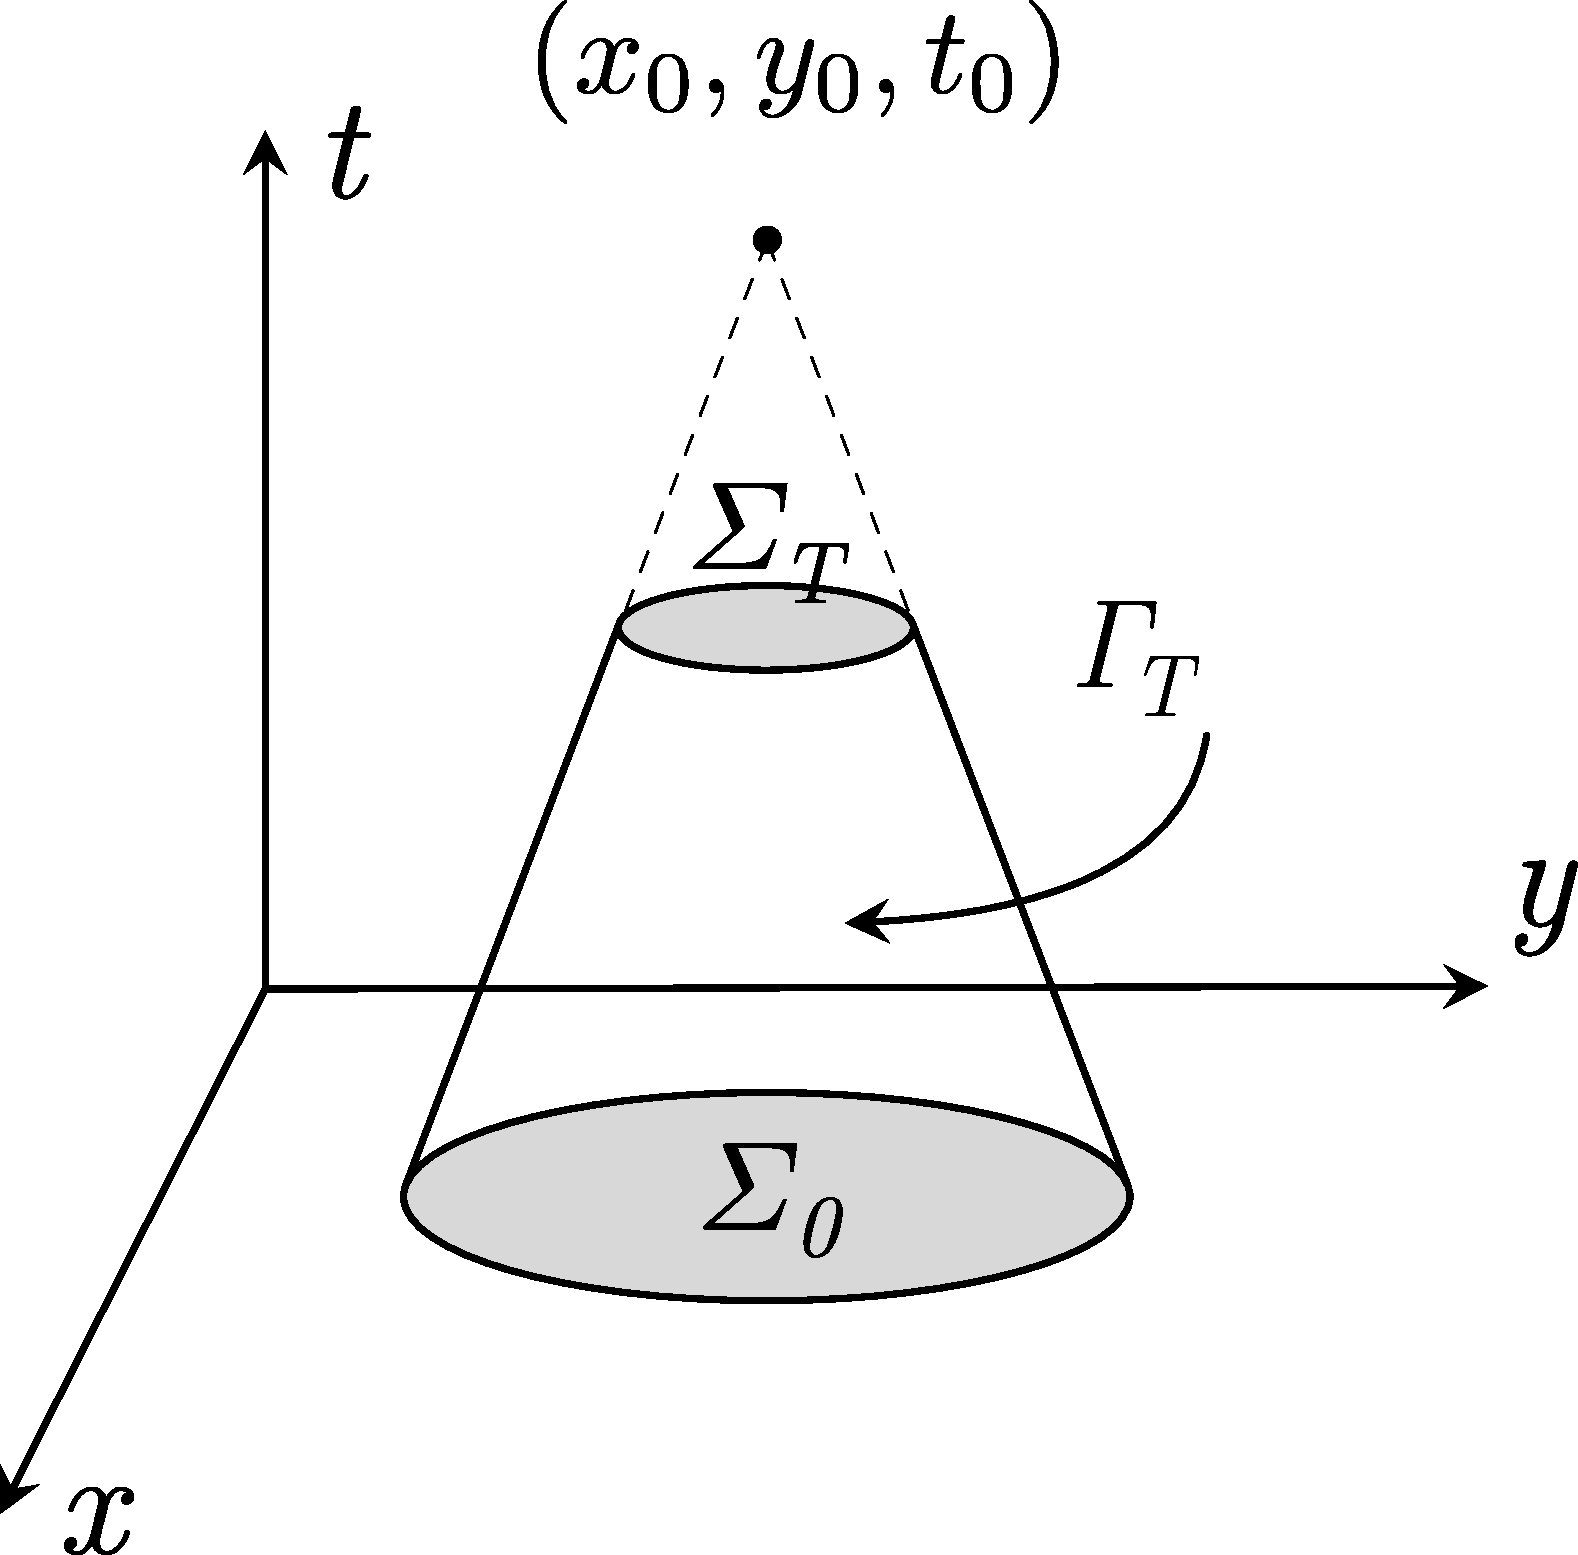
\includegraphics[width=0.28\linewidth]{./pic 10.pdf}
\end{center}
Вектор (внешней) нормали $ \vec{n} $ к этому усеченному конусу:
\begin{itemize}
	\item на $\Sigma_T:\ \vec{n} = \begin{pmatrix}1 & 0 & 0\end{pmatrix}^T $
	
	\item на $\Sigma_0:\ \vec{n} = \begin{pmatrix}-1 & 0 & 0\end{pmatrix}^T $
	
	\item на $\Gamma_T:\ \vec{n}=\dfrac{-1}{\sqrt{w_t^2+w^2_x+w^2_y}}
  \begin{pmatrix} w_t \\ w_x \\ w_y \end{pmatrix} =
  \begin{pmatrix} n_t \\ n_x \\ n_y \end{pmatrix}
  $
  \vspace{0.5em}

  В силу уравнения характеристик $\; w_t^2 - a^2w^2_x - a^2w^2_y = 0 \;$ (задаёт конус) имеем

  $n^2_t = a^2 \brk*{n^2_x + n^2_y}$\\
  $n^2_t + n^2_x + n^2_y = 1 \quad \Rightarrow \quad n^2_t = \dfrac{a^2}{a^2 +1} \quad \Rightarrow\quad n_t = \dfrac{a}{\sqrt{a^2+1}}.$
\end{itemize}


Функция \imaginarySubsection{Интеграл энергии}
$ \psi = v_t(v_{tt}- a^2v_{xx} - a^2v_{yy})\; $ тождественно равна нулю.

Раскроем скобки:
\begin{flalign*}
  \qquad 0\;\; &= v_t v_{tt} - a^2 v_t v_{xx}-a^2 v_t v_{yy}= &&\\
  &=\frac{1}{2}\brk*{v^2_t}_t + a^2 v_x v_{xt}-\brk*{a^2 v_t v_x}_x + a^2 v_y v_{yt} - \brk*{a^2 v_t v_y}_y = &&\\ 
  &=\frac{1}{2}\brk*{v^2_t}_t - \brk*{a^2 v_t v_x}_x - \brk*{a^2 v_t v_y}_y + \brk*{\frac{1}{2}a^2v^2_x}_t+\brk*{\frac{1}{2}a^2v^2_y}_t = &&\\ 
  &=\brk*{\frac{v^2_t+a^2v^2_x+a^2v^2_y}{2}}_t+\brk*{-a^2 v_t v_x}_x + \brk*{-a^2 v_t v_y}_y = &&\\
  &= F^{(t)}_t + F^{(x)}_x + F^{(y)}_y = \div\vec{F},
\end{flalign*}
\qquad где введено поле $\vec{F}$.
\vspace{0.7em}

Проинтегрируем полученную дивергенцию по объему усеченного конуса:
\begin{multline*}
  0 = \iiint\limits_{V_T}\div\vec{F}\, dV =
  \oiint\limits_{\partial V_T}(\vec{F},\vec{n})\, dS 
  =\iint\limits_{\Sigma_T}\frac{v^2_t+a^2v^2_x+a^2v^2_y}{2}\, dS - \iint\limits_{\Sigma_0}\frac{v^2_t+a^2v^2_x+a^2v^2_y}{2}\, dS + \\[0.4em]
  + \frac{1}{2}\iint\limits_{\Gamma_T}\brk*{(v^2_t+a^2v^2_x+a^2v^2_y)n_t-2a^2v_tv_xn_x - 2a^2v_tv_yn_y}dS
  \ = \ E(\Sigma_T) - E(\Sigma_0) + E(\Gamma_T)
\end{multline*}

В силу условий $ \eval{v}_{t=0} = \eval{v_t}_{t=0} = 0$ \ имеем \ $ E(\Sigma_0)=0 $ \ (под интегралом тождественный ноль).

Тогда\, $ E(\Sigma_T)+E(\Gamma_T)=0 $.\: 
Кроме того, \ $ E(\Sigma_T)\geq 0 $ \ (под интегралом сумма квадратов).
\vspace{0.5em}

Покажем, что и $ E(\Gamma_T)\geq 0 $: разделим и домножим её на $ n_t=\dfrac{a}{\sqrt{a^2+1}} $
\begin{multline*}
  \frac{1}{2}\frac{\sqrt{a^2+1}}{a}\iint\limits_{\Gamma_T}\brk*{(v^2_t+a^2v^2_x+a^2v^2_y)n^2_t \; - \; 2a^2v_tv_xn_tn_x \; - \; 2a^2v_tv_yn_tn_y} dS = \\ \shoveleft{
  =\frac{1}{2}\frac{\sqrt{a^2+1}}{a}\iint\limits_{\Gamma_T} \Bigl( v^2_t \overbrace{a^2(n^2_x + n^2_y)}^\text{= $n_t^2$}\; + \; a^2v^2_xn^2_t \; + \; a^2v^2_yn^2_t\; - \; 2a^2v_tv_xn_tn_x \; - \; 2a^2 v_t v_y n_t n_y \Bigr)\, dS }\\
  = \frac{1}{2} a \sqrt{a^2+1} \iint\limits_{\Gamma_T} \brk*{(v_tn_x -v_xn_t)^2+(v_tn_y-v_yn_t)^2} dS \;\ \geq\ 0  
\end{multline*}

Значит,\; $ E(\Sigma_0)=E(\Sigma_T)=E(\Gamma_T)\equiv 0.$
\; Из $ E(\Sigma_T)\equiv 0 $ получаем: 
$$ v_t\equiv 0,\ v_x\equiv 0,\ v_y\equiv 0 \quad \Rightarrow \quad v = \text{const} = \eval{v}_{t=0} = 0 
$$
Это верно всюду внутри усеченного конуса.
Заметая такими конусами всё пространство, получим, что $ v \equiv 0 $.
\end{proof}
\end{document}